% \iffalse meta-comment
%
% Copyright (C) 2021 by Geraldo Xexéo
%
% This file may be distributed and/or modified under the
% conditions of the LaTeX Project Public License, either
% version 1.3 of this license or (at your option) any later
% version. The latest version of this license is in:
%
% http://www.latex-project.org/lppl.txt
%
% and version 1.3 or later is part of all distributions of
% LaTeX version 2005/12/01 or later.
%
% \fi
%
%
%\iffalse
%<package>\NeedsTeXFormat{LaTeX2e}
%<package>\def\tr@version{v0.8}
%<package>\ProvidesPackage{task-report}[2021/06/09 \tr@version task-report]
%<*driver>
\documentclass{ltxdoc}
\usepackage[T1]{fontenc}
\usepackage[utf8]{inputenc}
\usepackage{lmodern}
\usepackage{csquotes}
\usepackage[brazilian,english]{babel}
\usepackage{datetime}
\usepackage{graphicx}
\usepackage{indentfirst}
\setlength{\parskip}{0.5em}
\usepackage{marvosym}
\usepackage[backend=biber,style=alphabetic,natbib]{biblatex}
\usepackage[editing]{coop-writing}
\usepackage{task-report}
\setlength{\cfttasksnumwidth}{25pt}
\usepackage{hyperref}
\cwnamedef{xexeo}{red}{Xexéo}
%
\EnableCrossrefs
\CodelineIndex
\RecordChanges
%
\DoNotIndex{\def,\long,\edef,\xdef,\gdef,\let,\global}
\DoNotIndex{\begin,\AtEndDocument,\newcommand,\newcounter,\stepcounter}
\DoNotIndex{\immediate,\openout,\closeout,\message,\typeout}
\DoNotIndex{\section,\scshape,\arabic}
%
%
%
\title{Task Report \taskreportversion}
\author{Geraldo Xexéo}
\date{\today\ - \ \currenttime}
\GetFileInfo{task-report.sty}
%
\makeindex
\MakeShortVerb{\|}
\begin{document}
    \DocInput{task-report.dtx}
    \newpage
    \PrintChanges
    \newpage
    \PrintIndex
    \newpage
    \listoftasks
\end{document}
%</driver>
% \fi
%
% \CheckSum{228}
%
% \CharacterTable
%  {Upper-case    \A\B\C\D\E\F\G\H\I\J\K\L\M\N\O\P\Q\R\S\T\U\V\W\X\Y\Z
%   Lower-case    \a\b\c\d\e\f\g\h\i\j\k\l\m\n\o\p\q\r\s\t\u\v\w\x\y\z
%   Digits        \0\1\2\3\4\5\6\7\8\9
%   Exclamation   \!     Double quote  \"     Hash (number) \#
%   Dollar        \$     Percent       \%     Ampersand     \&
%   Acute accent  \'     Left paren    \(     Right paren   \)
%   Asterisk      \*     Plus          \+     Comma         \,
%   Minus         \-     Point         \.     Solidus       \/
%   Colon         \:     Semicolon     \;     Less than     \<
%   Equals        \=     Greater than  \>     Question mark \?
%   Commercial at \@     Left bracket  \[     Backslash     \\
%   Right bracket \]     Circumflex    \^     Underscore    \_
%   Grave accent  \`     Left brace    \{     Vertical bar  \|
%   Right brace   \}     Tilde         \~}
%
% \changes{v0.1}{2021/05/31}{First version}
% \changes{v0.2}{2021/05/31}{User can create new states}
% \changes{v0.3}{2021/05/31}{List of Tasks}
% \changes{v0.4}{2021/06/01}{Allows redefining field names}
% \changes{v0.5}{2021/06/01}{Allows redefining header and colon}
% \changes{v0.6}{2021/06/01}{Numbers in tasks and references}
% \changes{v0.7}{2021/06/06}{Memoir class (used abntex2) badly emulates tocloft}
%\changes{v0.8}{2021/06/09}{Coppetex classes with blamed tocloft}
%\maketitle
%
% \tableofcontents
%
%\section{Introduction}
%
% This package supports the maintenance and report of a task list..
%
%
% \section{How to use task-report}
%
% |task-report| is available as open source at \url{https://github.com/xexeo/task-report}. The stable distribution is in the folder |dist|, while the lastest, and unstable, will be in the root folder.
%
% The only file you really need, besides this manual, is
% |task-report.sty|. This should be in your \LaTeX\   path, such as in the same folder that your main |.tex| file.
%
% You can make suggestions, complain about bugs, and request features using GitHub's ``Issues'' feature, in \url{https://github.com/xexeo/task-report/issues} (you must be signed in).
%
% \subsection{Using from Overleaf}
%
% The best way to use |task-report| inside Overleaf is to link
% the distributed style file through its URL. To do that, inside your project, select first ``Upload''. An ``Add files'' window will appear, then select ``From Externa URL'' and enter \url{https://raw.githubusercontent.com/xexeo/task-report/main/dist/task-report.sty} as ``URL to fetch the file from'' and ``task-report'' as ``File Name in This Project'', as in Figure \ref{fig:overleaffileurl}.
%
%\begin{figure}[tbh]
%    \centering
%    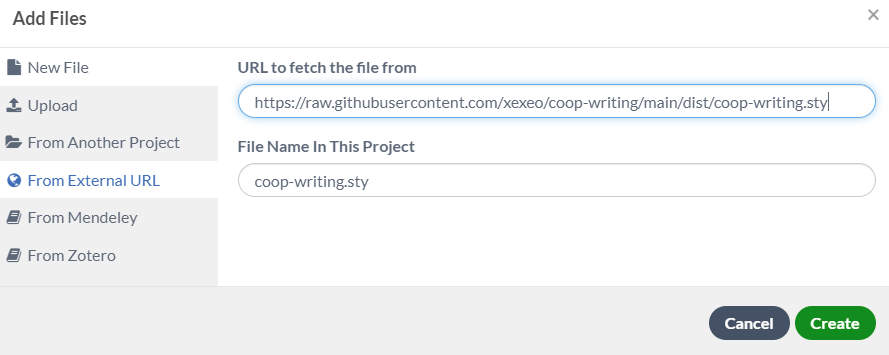
\includegraphics[width=0.9\linewidth]{images/overleaffileurl}
%    \caption{How to link a task-report.sty file in your project folder in Overleaf to the official distribution.}
%    \label{fig:overleaffileurl}
%\end{figure}
%
%
% \section{Package Options}
%
% \DescribeMacro{showtasknumbers} show tasks numbers, default is false.
%
% Users should never refer to a task by its number, since it can change from
% compilation to compilation if any task is inserted in among the existing ones.
% It is possible to use the |\label| macro to refer to tasks by number, page ou name.
%
% \subsection{General behavior}
%
%
%\section{Version}
%
% It is possible that the user wants to know the version
% being used. We provide two commands for it.
%
% \DescribeMacro{\taskreportversion}
% Provides the current version
%
% \DescribeMacro{\printtaskreportversion}
% Provides name and version
%
%
% |\taskreportversion| was used in the title of this article. The current version is \taskreportversion.
%
% If needed, the second macro prints also the name of the
% package:
%
%|\printtaskreportversion|
%
% will result in:
%
%\printtaskreportversion
%
% Please state the version when reporting bugs.
%
%
% \section{Usage}
%
% \DescribeMacro{\trtask}
% This is the main macro for the package.
%|\trtask|\oarg{status}\marg{name}\marg{due date}\marg{when-assigned}
% \marg{who-assigned}\marg{to-who-assigned}
% \marg{why}
% \marg{when-done}
% \marg{extra-text}
%
% Altough it has 8 arguments parameters, all of them can be empty. It has 9 arguments because this is the standard \LaTeX\  maximum.
%
% There are 5 possible standard states that are associated with a color (\textit{default color}): todo (red), doing(yellow), tocheck (cyan), checking (blue), and done(green). There is a pseudo-state other (black) that will be the color of any other word used of a state. Colors belong to the |xcolor| package and are configurable, as explained in section \ref{sec:conf}.
%
% The example:
%\begin{verbatim}
%\trtask[todo]{Make coffe}{Soon}{\today}{Geraldo Xexéo}{}{}{}{Please do the coffe strong}
%\trtask[doing]{Drink a coffe}{In 5 days}{June, 1st 2021}{The Boss}{The Worker}{}{}{}
%\trtask[tocheck]{Roast the beef}{}{June, 1st 2021}{The Boss}{The Worker}{}{\today}{Rare, plese}
%\trtask[checking]{Drink another beer}{}{June, 1st 2021}{The Boss}{The Worker}{}{\today}{Please check if you have age to drink in your country. If not, drink orangejuice.}
%\trtask[done]{Drink a beer}{}{\today}{The Boss}{The Worker}{Because I want}{\today}{}
%\trtask{}{}{}{}{}{}{}{}
%\trtask[done]{}{}{}{}{}{}{}{}
%\trtask[arg 1]{arg 2}{arg 3}{arg 4}{arg 5}{arg 6}{arg 7}{arg 8}{arg 9}
%\end{verbatim}
% generates:
%
%\trtask[todo]{Make coffe}{Soon}{\today}{Geraldo Xexéo}{}{}{}{Please do the coffe strong}
%\trtask[doing]{Drink a coffe}{In 5 days}{June, 1st 2021}{The Boss}{The Worker}{}{}{}
%\trtask[tocheck]{Roast the beef}{}{June, 1st 2021}{The Boss}{The Worker}{}{\today}{Rare, plese}
%\trtask[checking]{Drink another beer}{}{June, 1st 2021}{The Boss}{The Worker}{}{\today}{Please check if you have age to drink in your country. If not, drink orangejuice.}
%\trtask[done]{Drink a beer}{}{\today}{The Boss}{The Worker}{Because I want}{\today}{}
%\trtask{}{}{}{}{}{}{}{}
%\trtask[done]{}{}{}{}{}{}{}{}
%\trtask[arg 1]{arg 2}{arg 3}{arg 4}{arg 5}{arg 6}{arg 7}{arg 8}{arg 9}
%
%
% \section{Configuration}
%
% \subsection{Configuring Colors}
%\label{sec:conf}
% \DescribeMacro{\trsetboxcolors}
%% Set the colors for the 6 types of standard states
% Black otherwise.
%
% |\trsetboxcolors|\marg{todo-color}\marg{doing-color}\marg{tocheck-color}\marg{checking-color}
%\marg{done-color}\marg{other-color}
%
% The example:
%
%\begin{verbatim}
%\trsetboxcolors{magenta}{purple}{orange}{pink}{lime}{pink}
%
%\trtask[todo]{Drink a coffe}{next day}{\today}{The Boss}{The Worker}%
%{To keep awake}{\today}{Coffe must be strong and add 1 spoon of sugar}
%\trtask[doing]{Drink a coffe}{next day}{\today}{The Boss}{The Worker}%
%{To keep awake}{\today}{Coffe must be strong and add 1 spoon of sugar}
%\trtask[tocheck]{Drink a coffe}{next day}{\today}{The Boss}{The Worker}%
%{To keep awake}{\today}{Coffe must be strong and add 1 spoon of sugar}
%\trtask[checking]{Drink a coffe}{next day}{\today}{The Boss}{The Worker}%
%{To keep awake}{\today}{Coffe must be strong and add 1 spoon of sugar}
%\trtask[done]{Drink a coffe}{next day}{\today}{The Boss}{The Worker}%
%{To keep awake}{\today}{Coffe must be strong and add 1 spoon of sugar}
%\trtask{Drink a coffe}{\today}{next day}{The Boss}{The Worker}%
%{To keep awake}{\today}{Coffe must be strong and add 1 spoon of sugar}
%\end{verbatim}
%
% generates:
%
%\trsetboxcolors{magenta}{purple}{orange}{pink}{lime}{pink}
%
%\trsetboxcolors{magenta}{purple}{orange}{pink}{lime}{pink}
%
%\trtask[todo]{Drink a coffe}{next day}{\today}{The Boss}{The Worker}%
%{To keep awake}{\today}{Coffe must be strong and add 1 spoon of sugar}
%\trtask[doing]{Drink a coffe}{next day}{\today}{The Boss}{The Worker}%
%{To keep awake}{\today}{Coffe must be strong and add 1 spoon of sugar}
%\trtask[tocheck]{Drink a coffe}{next day}{\today}{The Boss}{The Worker}%
%{To keep awake}{\today}{Coffe must be strong and add 1 spoon of sugar}
%\trtask[checking]{Drink a coffe}{next day}{\today}{The Boss}{The Worker}%
%{To keep awake}{\today}{Coffe must be strong and add 1 spoon of sugar}
%\trtask[done]{Drink a coffe}{next day}{\today}{The Boss}{The Worker}%
%{To keep awake}{\today}{Coffe must be strong and add 1 spoon of sugar}
%\trtask{Drink a coffe}{\today}{next day}{The Boss}{The Worker}%
%{To keep awake}{\today}{Coffe must be strong and add 1 spoon of sugar}
%
%
%\trsetboxcolors{red}{yellow}{cyan}{blue}{green}{black}
%
%
% \subsection{Changing Field Names}
%
% You can change all field names with command \DescribeMacro{\trsetfieldsnames}. % This command can be used to internationalization or to make these box used by any other reason.
%
%
% |\trsetfieldsnames|\marg{status}\marg{duedate}\marg{assigned}
% \marg{from}\marg{to}
% \marg{done}\marg{why}
%
%
% For example:
%
%\begin{verbatim}
%\trsetfieldsnames{Stage}{Must be ready in}{Demand date}{Who asked for}{To who}{Ready in}{Reasons}
%\trtask[done]{Drink a coffe}{5 days}{\today}{The Boss}{The Worker}%
%{To keep awake}{\today}{Coffe must be strong and add 1 spoon of sugar}
%\end{verbatim}
%
% generates:
%
%\trsetfieldsnames{Stage}{Must be ready in}{Demand date}{Who asked for}{To who}{Ready in}{Reasons}
%\trtask[done]{Drink a coffe}{5 days}{\today}{The Boss}{The Worker}%
%{To keep awake}{\today}{Coffe must be strong and add 1 spoon of sugar}
%
%
%\trsetfieldsnames{Status}{Due date}{Assigned in}{From}{To}{Done in}{Rationale}
%
%
% \subsection{Modifying the Header}
%
% \DescribeMacro{\trsettitlelabel} Sets the label for the header.
%
% |\trsettitlelabel|\marg{label-for-header}
%
%\begin{verbatim}
% \trsettitlelabel{Task}
%
%\trtask[done]{Drink a coffe}{5 days}{\today}{The Boss}{The Worker}
%{To keep awake}{\today}{Coffe must be strong and add 1 spoon of sugar}
%
%\end{verbatim}
%
% \trsettitlelabel{Task}
%
%\trtask[done]{Drink a coffe}{5 days}{\today}{The Boss}{The Worker}
%{To keep awake}{\today}{Coffe must be strong and add 1 spoon of sugar}
%
% Back to normal:
%
%\begin{verbatim}
% \trsettitlelabel{}
%
%\trtask[done]{Drink a coffe}{5 days}{\today}{The Boss}{The Worker}
%{To keep awake}{\today}{Coffe must be strong and add 1 spoon of sugar}
%\end{verbatim}
%
%
% \trsettitlelabel{}
%
%\trtask[done]{Drink a coffe}{5 days}{\today}{The Boss}{The Worker}
%{To keep awake}{\today}{Coffe must be strong and add 1 spoon of sugar}
%
% \subsection{Creating New States}
%
% Users can create their own state using  \DescribeMacro{\traddstatecolor}
%
% |\traddstatecolor|\marg{state}\marg{color}
%
% For example:
%
%\begin{verbatim}
%\traddstatecolor{waiting}{teal}
%\trtask[waiting]{Drink a coffe}{\today}{The Boss}{The Worker}%
%{To keep awake}{\today}{Coffe must be strong and add 1 spoon of sugar}
%\end{verbatim}
%
% generates:
%
%\traddstatecolor{waiting}{teal}
%\trtask[waiting]{Drink a coffe}{ASAP}{\today}%
%{The Boss}{The Worker}%
%{To keep awake}{\today}{Coffe must be strong and add 1 spoon of sugar}
%
% \section{Using Labels to Refer to Tasks}
%
%  You can use labels, such as |\label{task:kanbam}| \textbf{in the last}
% \textbf{argument}\footnote{Actually, they will probably break only if used in the second argument, that is used to name them} and refer to it with commands |\ref{task:kanbam}| (\ref{task:kanbam}),
%|\pageref{task:kanbam}| (\pageref{task:kanbam}) ou |\nameref{task:kanbam}|
% (\nameref{task:kanbam}).
%
%
% \section{The List of Tasks}
%
% \DescribeMacro{\listoftasks}
% A list of tasks can be generated with the command:
%
% |\listoftasks|
%
%
% Its title can be changed with the command:
%
% |\trsettasklisttitle|\marg{new-title}
%
% The command:
%
% |\setlength{\cfttasksnumwidth}{25pt}|
%
% from package |tocloft| can be used to set the space used by
% the section indicator.
%
%
%
%\section{Warnings}
% This package uses another package that changes \LaTeX's standard behavior for summary and lists. When you use it, you must explicitly change pages with |\newpage|
% before |\tableofcontents| or similar commands.
%
% \section{Implementation}
%
% \StopEventually{End of Code}
%
% \subsection{Options}
% \DescribeMacro{showtasknumbers}
%
% Since task numbers can change between compilations
% this default is set to |false|.
%
%    \begin{macrocode}
\newif\if@showtasknumbers\@showtasknumbersfalse%
\newif\if@cwtoclofttitles\@cwtoclofttitlesfalse
%
\DeclareOption{showtasknumbers}{\@showtasknumberstrue}%
\DeclareOption{toclofttitles}{\@cwtoclofttitlestrue}
%
\ProcessOptions\relax
%    \end{macrocode}
%
% \subsection{Required Packages}
%
%
%\begin{itemize}
%    \item |mdframed| makes the frame aroung tasks
%    \item |etoolbox| command ifstringempty
%    \item |tocloft|  create the list of tasks
%\end{itemize}
%
% Must defend coppe against tocloft
%
%    \begin{macrocode}
\RequirePackage{tcolorbox}%
\RequirePackage{etoolbox}%
\@ifclassloaded{coppe}%
{%
    \RequirePackage[titles]{tocloft}%
}%
{%
    \if@cwtoclofttitles%
    \RequirePackage[titles]{tocloft}%
    \else%
    \RequirePackage{tocloft}%
    \fi%
}%
\RequirePackage{hyperref}%
%    \end{macrocode}
% \subsection{Solving problems with other packages}
%
% \subsubsection{Problems with \texttt{abntex2} and \texttt{memoir}}
%
% |abntex2| causes error in |\newlistof|, you
% can't refer to |chapter|, |section| or other counter
% as optional argument
%
% This error is actually |memoir| fault\pleasecite[memoir package], since it emulates
% |tocloft| (and other packages). I can´t imagine why...
%
% Therefore, we will avoid using the command with option
% when the class is present
%
%    \begin{macrocode}
\@ifclassloaded{memoir}%
{% TRUE
    \newif\if@cwmemoirdefense\@cwmemoirdefensetrue%
}%
{% FALSE
    \newif\if@cwmemoirdefense\@cwmemoirdefensefalse%
}%
%
%    \end{macrocode}%
% \subsection{Access to the current version}
% We provide some macros for the user to know the version being used.
% \begin{macro}{\taskreportversion}
% Provides current version of coop-writing
%    \begin{macrocode}
\newcommand{\taskreportversion}{\tr@version}%
%    \end{macrocode}
% \end{macro}
%
% \begin{macro}{\printtaskreportversion}
% Provides package name and version
%    \begin{macrocode}
\newcommand{\printtaskreportversion}{task-report \taskreportversion}%
%    \end{macrocode}
% \end{macro}
%
% \subsection{Color Management for States}
%
% \subsection{Defining States Through a Simulated List}
%
% \begin{macro}{\traddstatecolor}
% \begin{macro}{\usestatecolor}
%
% Inserts states and their colors in a simulated list and uses them
%
%    \begin{macrocode}
\newcommand{\traddstatecolor}[2]{%
    \@ifundefined{\string\color@#2}%
    {%
        \message{#2 not defined}%
        \expandafter\ERROR%
    }%
    {%
        \expandafter\gdef\csname tr@astate@\detokenize{#1}\endcsname{#2}%
}%
}%
%
\def\tr@usestatecolor#1{%
    \ifcsname tr@astate@\detokenize{#1}\endcsname%
    \csname tr@astate@\detokenize{#1}\expandafter\endcsname%
    \else%
\tr@astate@other%
    \fi%
}%
%    \end{macrocode}
% \end{macro}
% \end{macro}
%
% \begin{macro}{\trsetboxcolors}
%
% Set the colors for the 6 types of standard states
% Black otherwise.
%
% |\trsetboxcolors|\marg{todo-color}\marg{doing-color}
% \marg{tocheck-color}\marg{checking-color}
% \marg{done-color}\marg{other-color}
%
%    \begin{macrocode}
\newcommand{\trsetboxcolors}[6]{%
\traddstatecolor{todo}{#1}
\traddstatecolor{doing}{#2}
\traddstatecolor{tocheck}{#3}
\traddstatecolor{checking}{#4}
\traddstatecolor{done}{#5}
\traddstatecolor{other}{#6}
}%
%    \end{macrocode}
% \end{macro}
% \subsection{Standard Colors}
%
% Sets the standard colors for the standard states
%
%    \begin{macrocode}
\trsetboxcolors{red}{yellow}{cyan}{blue}{green}{black}
%    \end{macrocode}
%
%
% \subsection{Managing The Fields Names}
%
% \begin{macro}{\traddfieldname}
% \begin{macro}{\tr@usesfieldname}
%
% Define field names - does not create a new field
%
%    \begin{macrocode}
\newcommand{\traddfieldname}[2]{%
    \expandafter\gdef\csname tr@fieldnames@\detokenize{#1}\endcsname{#2}%
}%
%
\def\tr@usesfieldname#1{%
    \ifcsname tr@fieldnames@\detokenize{#1}\endcsname%
    \csname tr@fieldnames@\detokenize{#1}\expandafter\endcsname%
    \else%
Missing Field Name%
    \fi%
}%
%    \end{macrocode}
% \end{macro}
% \end{macro}
%
% \subsection{Standard Field Names}
%
% Sets the standard text for the fields
%
% \begin{macro}{\trsetfieldsnames}
% \begin{macro}{\trsettitlelabel}
%
% Set the names for the field names and for the titles.
%
% |\trsetfieldsnames|\marg{status}\marg{duedate}\marg{assigned}
% \marg{from}\marg{to}
% \marg{done}\marg{why}
%
% |\trsettitlelabel|\marg{title-label}
%
%    \begin{macrocode}
\newcommand{\trsetfieldsnames}[7]{%
    \traddfieldname{status}{#1}%
    \traddfieldname{duedate}{#2}%
    \traddfieldname{assigned}{#3}%
    \traddfieldname{from}{#4}%
    \traddfieldname{to}{#5}%
    \traddfieldname{done}{#6}%
    \traddfieldname{why}{#7}%
}%
%
\traddfieldname{defaulttitle}{Task without a name}%
%
\def\tr@defaulttitlelabel{}%
\newcommand{\trsettitlelabel}[1]{%
    \def\tr@defaulttitlelabel{#1}%
}%
%
\trsetfieldsnames{Status}{Due date}{Assigned in}{From}{To}{Done in}{Rationale}
%
%    \end{macrocode}
%
% \end{macro}
% \end{macro}
%
%
% \begin{macro}{\trsetcolon}
%    \begin{macrocode}
\newcommand{\trsetcolon}[1]{%
    \traddfieldname{colonmark}{#1}
}
\trsetcolon{:}
%    \end{macrocode}
% \end{macro}
%
%
%
% \begin{macro}{\tr@currentboxcolor}
%
% The dirt trick of using a global variable to
% store a value
%
%    \begin{macrocode}
\def\tr@currentboxcolor{\tr@usestatecolor{other}}%
%    \end{macrocode}
% \end{macro}
%
%
%
% \begin{macro}{\trstatuscolor}
%
% Select the color based on the state
%
% |\trstatuscolor|\marg{state}
%
%    \begin{macrocode}
\newcommand{\trstatuscolor}[1]%
{%
\ifblank{#1}%
{%
\def\tr@currentboxcolor{\tr@usestatecolor{other}}%
}%
{%
\def\tr@currentboxcolor{\tr@usestatecolor{#1}}%
}%
}%
%    \end{macrocode}
% \end{macro}
%
%
% \subsection{List of Tasks}
%    \begin{macrocode}
\newcommand{\trsettasklisttitle}[1]{%
    \def\trlisttasks{#1}%
}%
\trsettasklisttitle{List of Tasks}%
%% cria a lista, depende do pacoto tcloft
\if@cwmemoirdefense%
\@ifundefined{chapter}%
{\newlistentry[section]{tasks}{trt}{0}}%
{\newlistentry[chapter]{tasks}{trt}{0}}%
\newlistof{listoftasks}{trt}{\trlisttasks}%
\else%
\@ifundefined{chapter}%
{\newlistof[section]{tasks}{trt}{\trlisttasks}}%
{\newlistof[chapter]{tasks}{trt}{\trlisttasks}}%
\fi%
%    \end{macrocode}
%
% \subsection{Declaring Tasks}
%
% \subsubsection{Helpers}
%
% \begin{macro}{\tr@field}
%
% Helpers to build the task
% |\trtitle| should be improved to chack if
% |\tr@defaulttitlelabel| is not empty and use it
%
%    \begin{macrocode}
\newcommand{\tr@title}[2]{%
\ifx\tr@defaulttitlelabel\empty%
    \if@showtasknumbers%
        \textbf{#2\tr@usesfieldname{colonmark} #1}%
    \else%
        \textbf{#1}%
    \fi%
\else%
    \if@showtasknumbers%
        \textbf{\tr@defaulttitlelabel\ #2\tr@usesfieldname{colonmark}\  #1}%
    \else%
        \textbf{\tr@defaulttitlelabel\tr@usesfieldname{colonmark}\  #1}%
    \fi%
\fi%
}%
%
\newcommand{\tr@field}[2]{%
\textbf{#1}\tr@usesfieldname{colonmark} #2%
}%
%
%    \end{macrocode}
% \end{macro}
%
% \subsubsection{Main task macro}
%
% \begin{macro}{\trtask}
%
%  Describes a task
%
%|\trtask|\oarg{status}\marg{name}\marg{due-date}
% \marg{when-assigned} \marg{who-assigned}
% \marg{to-who-assigned}\marg{why}
% \marg{when-done}\marg{extra-text}
%
% For example:
%\begin{verbatim}
%\trtask[doing]{Make a \LaTeX\ Kanbam document}{soon}
% {2021-05-31}{Xexéo}{Geraldo Xexéo}{Help control tasks}
% {not yet}{Use colors\label{task:kanbam}}
%\end{verbatim}
%
% generates:
%
%\trtask[doing]{Make a \LaTeX\ Kanbam document}{soon}
% {2021-05-31}{Xexéo}{Geraldo Xexéo}{Help control tasks}
% {not yet}{Use colors\label{task:kanbam}}
%
% It is possible to reference the task (as Task \ref{task:kanbam} in page \pageref{task:kanbam}, named \nameref{task:kanbam}).
%
%    \begin{macrocode}
%  [status] , what, due-date when-assigned, from-who, to-who, why, when-done, extra
\newcounter{taskcounter}
%
\newcommand{\trtask}[9][]{%
    \par%
    \ifblank{#2}{
    \def\trtask@temp{\tr@usesfieldname{defaulttitle}}%
    }%
    {%
    \def\trtask@temp{#2}%
    }%
    \refstepcounter{tasks}%
% \refstepcounter updates \@currentlabel (\LaTeX magic!)
% therefore the next command must appear before #9, where label must be.
    \refstepcounter{taskcounter}%
    \protected@edef\@currentlabelname{\trtask@temp}% trying to make it work
    \addcontentsline{trt}{tasks}{\protect\numberline{\thetasks}{\trtask@temp}}%
    \trstatuscolor{#1}%
    \begin{tcolorbox}[title=\tr@title{\trtask@temp}{\thetaskcounter},%
colback=\tr@currentboxcolor!5!white,%
colframe=\tr@currentboxcolor!75!black%
]%
        \ifblank{#1}{}%
        {%
            \tr@field{\tr@usesfieldname{status}}{#1}\newline%
        }%
        \ifblank{#3}{}%
{%
    \tr@field{\tr@usesfieldname{duedate}}{#3}\newline%
}%
\ifblank{#4}{}%
{%
    \tr@field{\tr@usesfieldname{assigned}}{#4}\newline%
}%
\ifblank{#5}{}%
{%
    \tr@field{\tr@usesfieldname{from}}{#5}\newline%
}%
\ifblank{#6}{}%
{%
    \tr@field{\tr@usesfieldname{to}}{#6}\newline%
}%
\ifblank{#7}{}%
{%
    \tr@field{\tr@usesfieldname{why}}{#7}\newline%
}%
\ifblank{#8}{}%
{%
    \tr@field{\tr@usesfieldname{done}}{#8}\newline%
}%
        \ifblank{#9}{}%
        {\tcblower%
        #9%
        }%
    \end{tcolorbox}%
}%
%    \end{macrocode}
% \end{macro}
%
%
%
%
% \Finale
%
% \endinput
% Local Variables:
% mode: doctex
% TeX-master: t
% End:
